\section{Logowanie i rejestracja}

Tworzony system wymaga identyfikacji użytkowników, więc aplikacje mobilne musiały zapewniać funkcjonalność logowania i rejestracji. 
Na rysunku \ref{fig:login} przedstawione zostały pierwsze ekrany tego procesu. Na początku nie jest określone, która dokładnie czynność jest wykonywana. Dopiero gdy użytkownik wybierze metodę uwierzytelnienia i poda swój login, to następuje sprawdzenie, czy ma on konto, czy nie i procedura od tego momentu jest kontynuowana odpowiednio jako logowanie lub rejestracja.

\begin{figure}[ht]
  \centering
  \begin{subfigure}[t]{0.33\textwidth}
    \centering
    \fbox{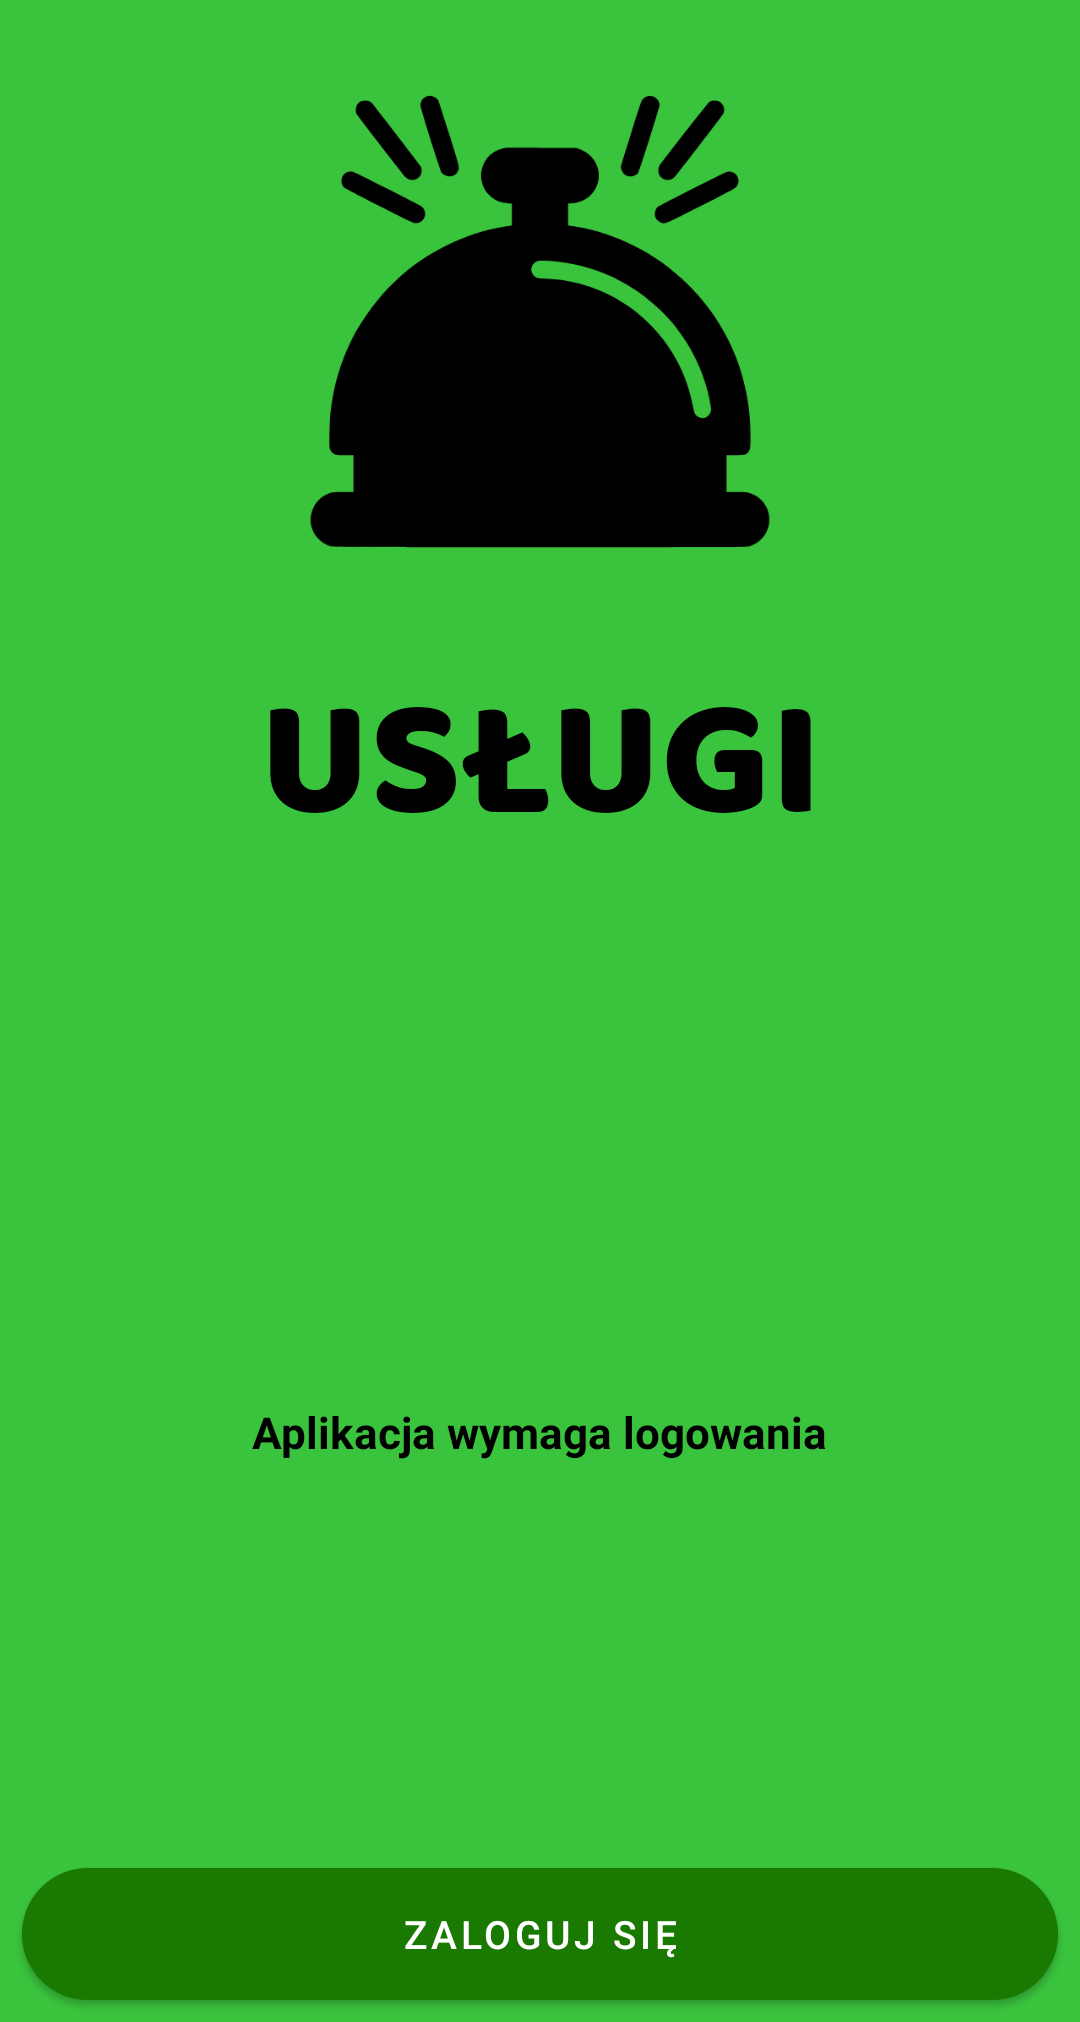
\includegraphics[width=0.97\linewidth]{screens/login_start.png}}
    \caption{Ekran rozpoczęcia}
  \end{subfigure}
  \begin{subfigure}[t]{0.33\textwidth}
    \centering
    \fbox{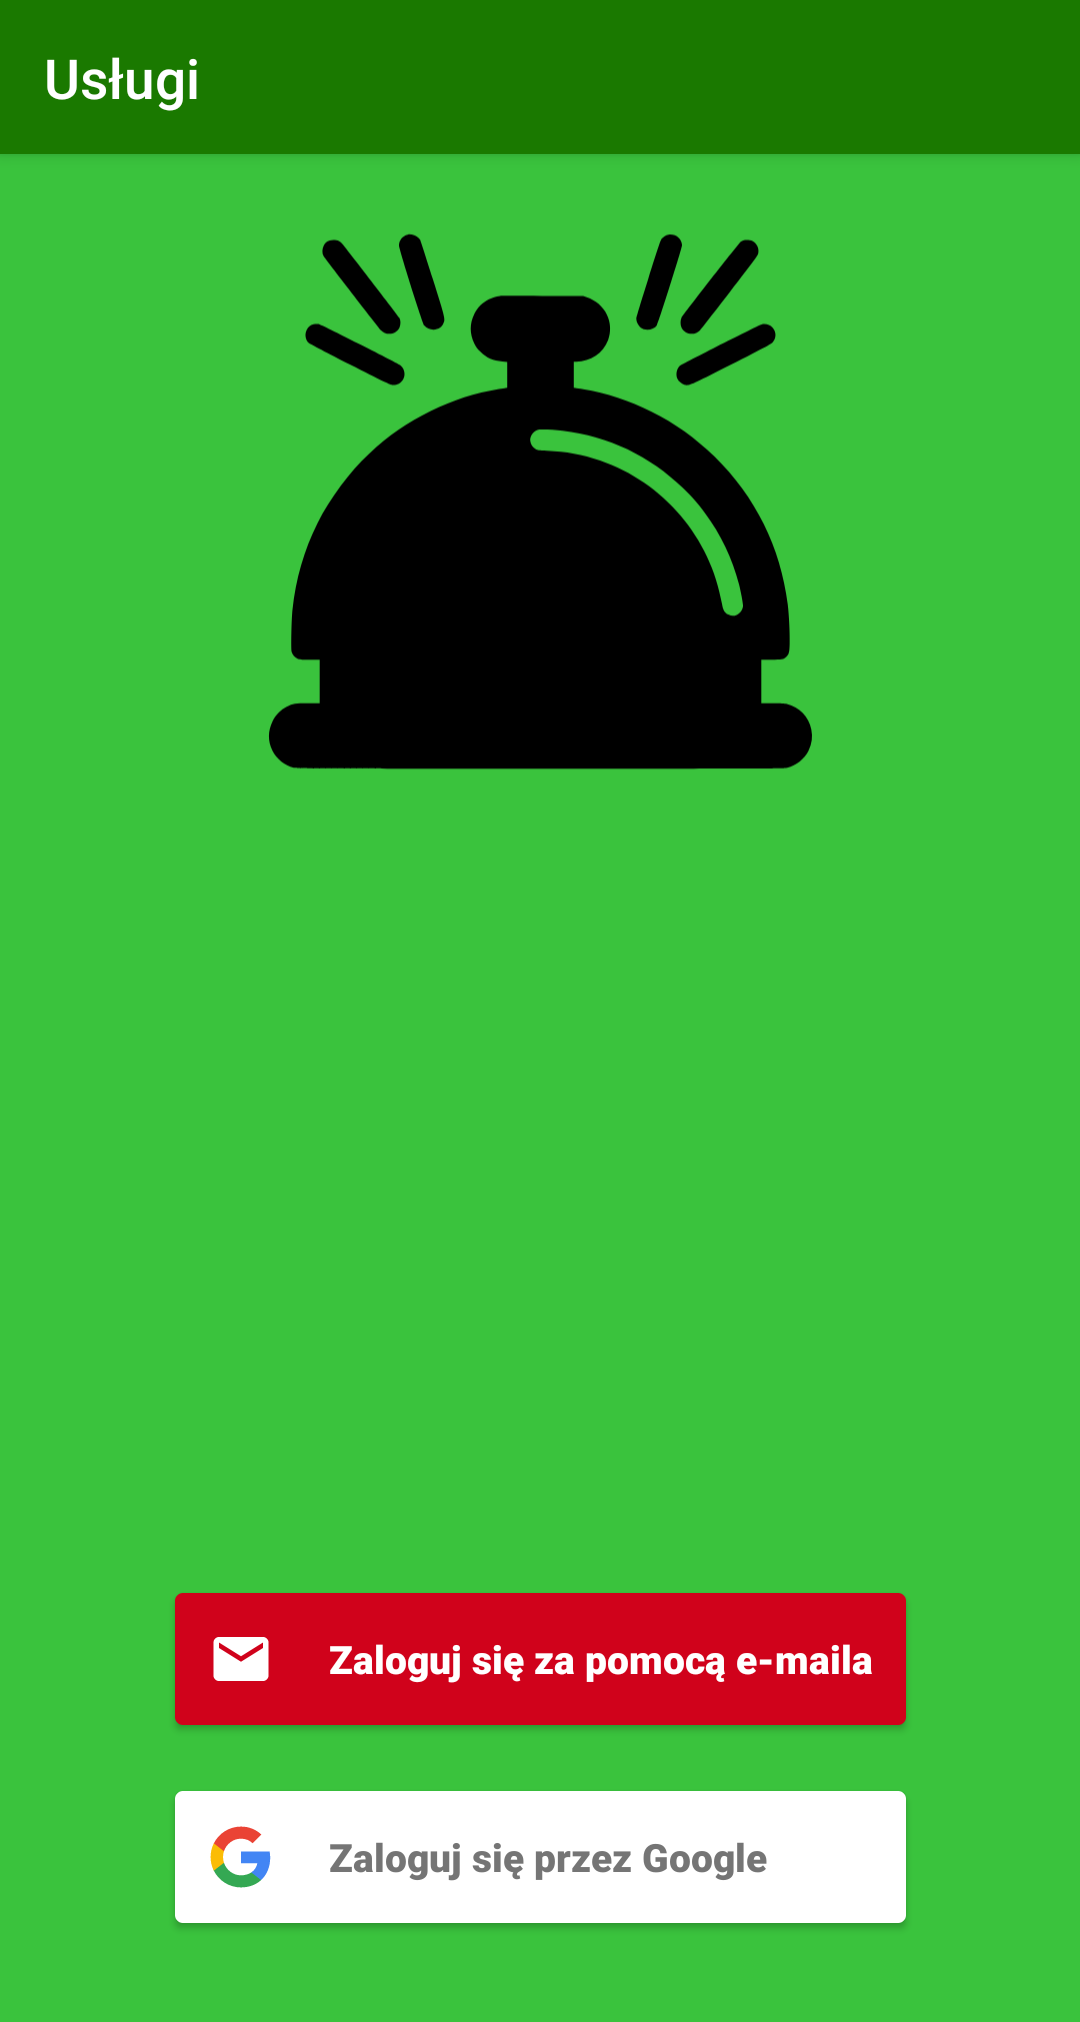
\includegraphics[width=0.97\linewidth]{screens/login_method.png}}
    \caption{Ekran wyboru metody}
  \end{subfigure}
  \caption{Pierwsze ekrany procesu autoryzacji}
  \label{fig:login}
\end{figure}

Wybierając metody autoryzacji sugerowano się publikacją \enquote{Investigating login features in smartphone apps} \cite{login-methods}, która analizuje związki pomiędzy dostępnymi w aplikacjach mobilnych metodami logowania, a ich popularnością. Wyciągnięto w niej wniosek, że obecność logowania społecznościowego jest jednym z czynników, który skłania użytkowników do wystawiania wyższych ocen. Wykorzystanie własnych systemów autoryzacji takiej właściwości już nie przejawia. Z tego powodu postanowiono wybrać ten rodzaj logowania, a dokładnie logowanie za pomocą Google, które z uwagi na wykorzystywaną już platformę Google Firebase okazało się proste w integracji. Kierując się jednak innym artykułem \cite{social-login}, klasyczne logowanie adresem e-mail również postanowiono wykorzystać. Wymienia on obawy dotyczące prywatności, utraty anonimowości i bezpieczeństwa jako zniechęcające ludzi do używania logowania społecznościowego. Został napisany dość dawno i przypuszcza się, że nie są one już tak bardzo powszechne, jednak wciąż spotykane.

Przy implementacji logowania i rejestracji po stronie aplikacji klienckich dominującą rolę odegrała biblioteka FirebaseUI, która dostarczyła niemalże gotowy szablon procesu autoryzacji. Po skonfigurowaniu metod logowania i wyglądu, by zapewnić spójność z resztą aplikacji, wygenerowała ona wszystkie potrzebne ekrany. Kierowała się przy tym najlepszymi znanymi praktykami. Ze względu na dużą ilość takich ekranów postanowiono nie prezentować ich wyglądu. Wykorzystują one funkcję Smart Lock w celu automatycznego logowania przy użyciu zapisanych wcześniej danych oraz obsługują kłopotliwe scenariusze, takie jak odzyskiwanie konta.
